\FloatBarrier

\begin{figure}[h!]
	\centering
	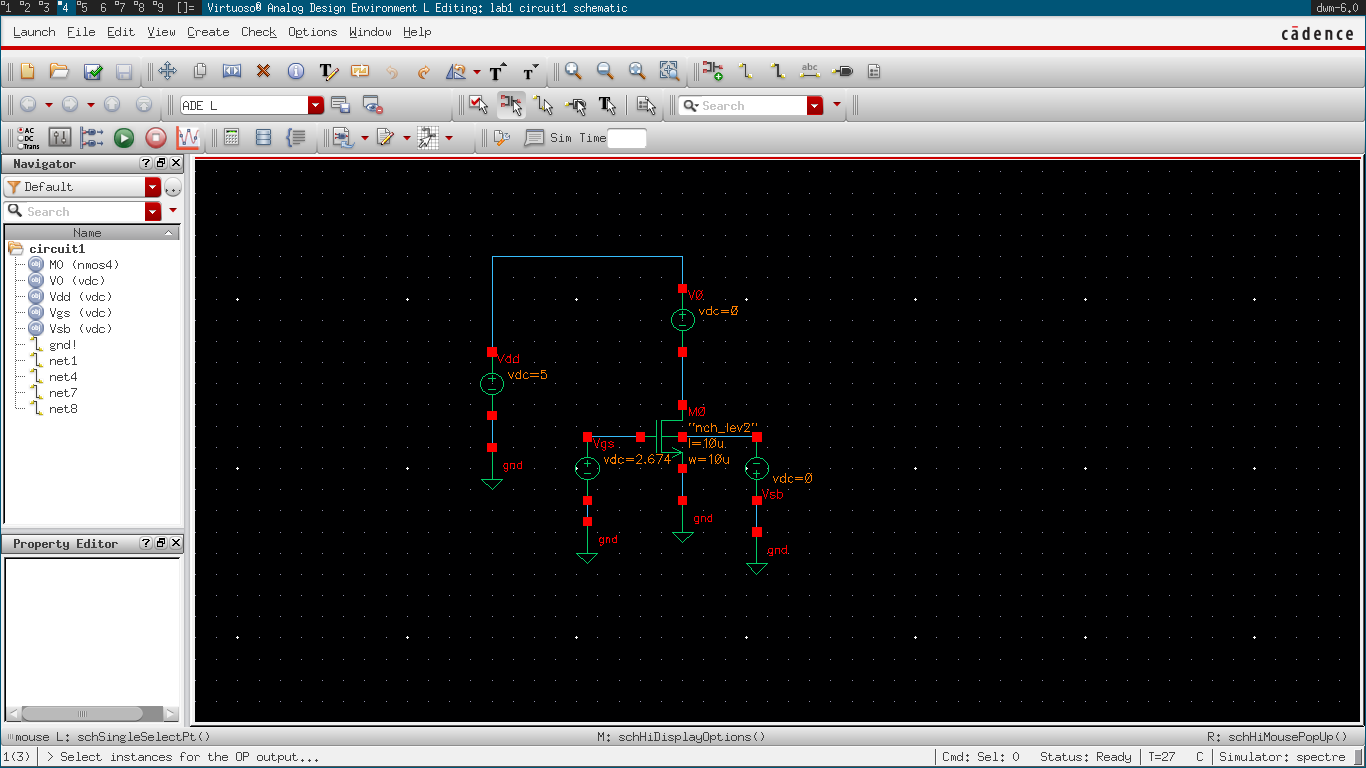
\includegraphics[scale=0.75]{../images/circuit1.PNG}
	\caption{Circuit for Simulation 1}
	\label{fig:circuit1}
\end{figure}

\FloatBarrier

The value of $V_{GS}$ for which $I_{D} = 500$\si{\micro\ampere} is determined in table (\ref{tab:sim1_results}).
$g_{m}$ is determined from a DC operating point analysis in Virtuoso.

\FloatBarrier

\begin{figure}[h!]
	\centering
	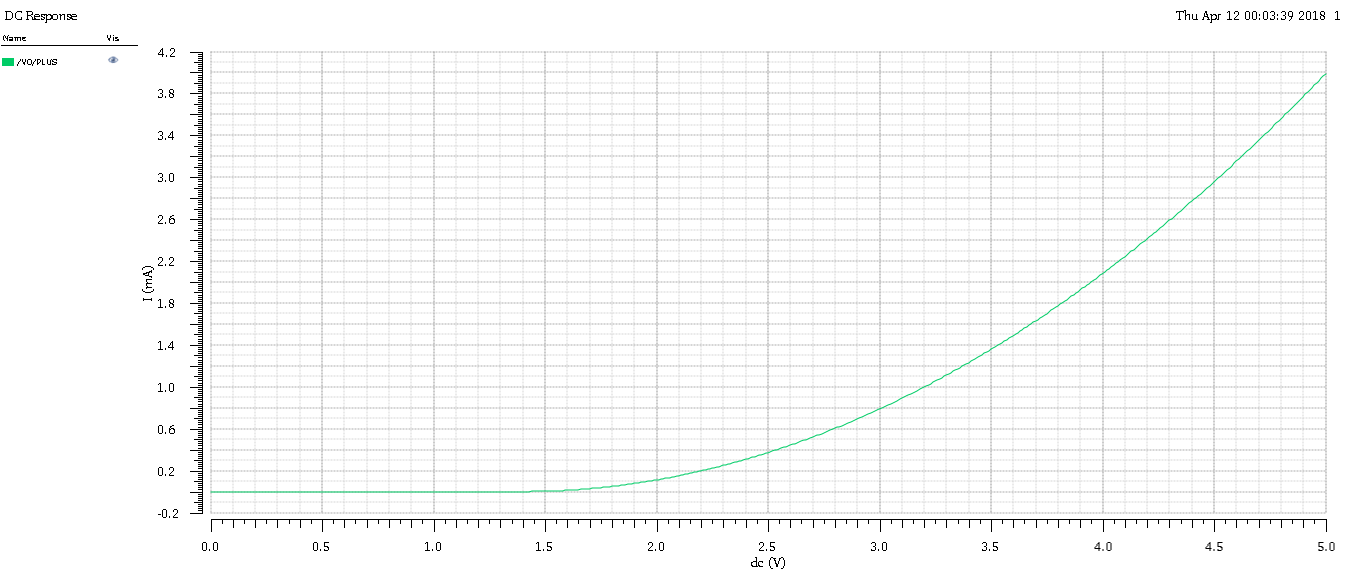
\includegraphics[scale=0.75]{../images/id_vs_vgs.PNG}
	\caption{$I_{D}$ versus $V_{GS}$ for NMOS}
	\label{fig:id_vs_vgs}
\end{figure}

\FloatBarrier

\FloatBarrier

\begin{figure}[h!]
	\centering
	\includegraphics[scale=0.75]{../images/did_vs_vgs.PNG}
	\caption{$\frac{I_{D}}{V_{GS}}$ versus $V_{GS}$ for NMOS}
	\label{fig:did_vs_vgs}
\end{figure}

\FloatBarrier

\FloatBarrier

\begin{table}[h!]
	\centering
	\caption{Simulation 1 Results}
	\label{tab:sim1_results}
	\csvautotabular{../tables/sim1_results.csv}
\end{table}

\FloatBarrier
